\chapter[Vierzig Jahre USCU]{Vierzig Jahre USCU -  Von der ungeheuren Lust auf bewegtes Wasser ... }
\label{cha:2}

\paragraph{Hoch über dem Lichtermeer der Stadt Ulm traf sich Mitte November 2017 eine ganz besondere Festgesellschaft. Der Saal in der Hochschule für Gestaltung (HfG) ist dekoriert mit nautischem Gerät und Ölzeug, ausgediente Seekarten schmücken die Tische für die 120 Gäste. So sieht es aus, wenn der Universitätssegelclub Ulm e.V. (USCU) seinen 40. Geburtstag feiert.}
Als Club „ohne Haus und Wasser“ wurde der USCU am 4. Juli 1977 geboren. Entstanden aus einer Segelgruppe des Studentensports hat er sich über die Jahre zu einer universitären Instanz entwickelt. Ob Studierende oder Professoren, Verwaltungsangestellte, Wissenschaftler oder Bürger aus der Stadt - alle verbindet sie eine besondere Leidenschaft: das Segeln. Der Uni-Segelverein versteht sich dabei im mehrfachen Sinn als Bildungseinrichtung: „In vierzig Jahren haben wir mehr als 4000 Sportboot-Segelscheine vergeben“, so der erste Vorsitzende Dr. Jürgen Hoppe in seiner Festrede. Dazu gehören Binnen-, Küsten- und Seeschifferscheine. Für die Persönlichkeitsbildung sei das Segeln ebenfalls hilfreich, fördere es doch Verantwortungssinn, Teamgeist und strategisches Denken. Und sogar die universitäre Lehre in der Botanik, der Zoologie und der Mikrobiologie profitiert vom ehrenamtlichen Engagement des USCU. 

„Seit 2001 gibt es regelmäßige Exkursionen für Biologen, die zum Modul 'Ökologie des Mittelmeerraumes' gehören und die ohne die seemännische Unterstützung durch Skipper des Vereins nie möglich gewesen wären“, erklärte der lehrerfahrene Biologe vom Institut für Systematische Botanik und Ökologie. So wuchs die Zahl der Mitglieder vom ersten Gründungsjahr bis heute von 49 auf über 350. Über den Hochschulsport kommen vor allem viele Studierende zum Verein, und auch das Studium Generale hat Ausbildungsangebote des USCU im Programm. 

Die Universität unterstützt den Segelclub, der seit letztem Jahr den Status einer Hochschulgruppe hat, mit Räumlichkeiten für die Theorieausbildung. Praktische Segelerfahrung sammeln die Kursteilnehmer je nach Schein auf dem Ammer- und Bodensee, im Mittelmeer oder an der Ostsee. Dafür kooperiert der USCU mit Segelschulen vor Ort. Am Bodensee hat der Verein seit einigen Jahren nun sogar ein vereinseigenes Boot mit Wasserliegeplatz: die Alpha32; eine 32 Fuß lange Segelyacht, hergestellt von der Firma Esslinger \& Abt in Laupheim. 

\begin{wrapfigure}{l}{0.48\textwidth} % um Bild von Text umfließen zu lassen
    \begin{center}
      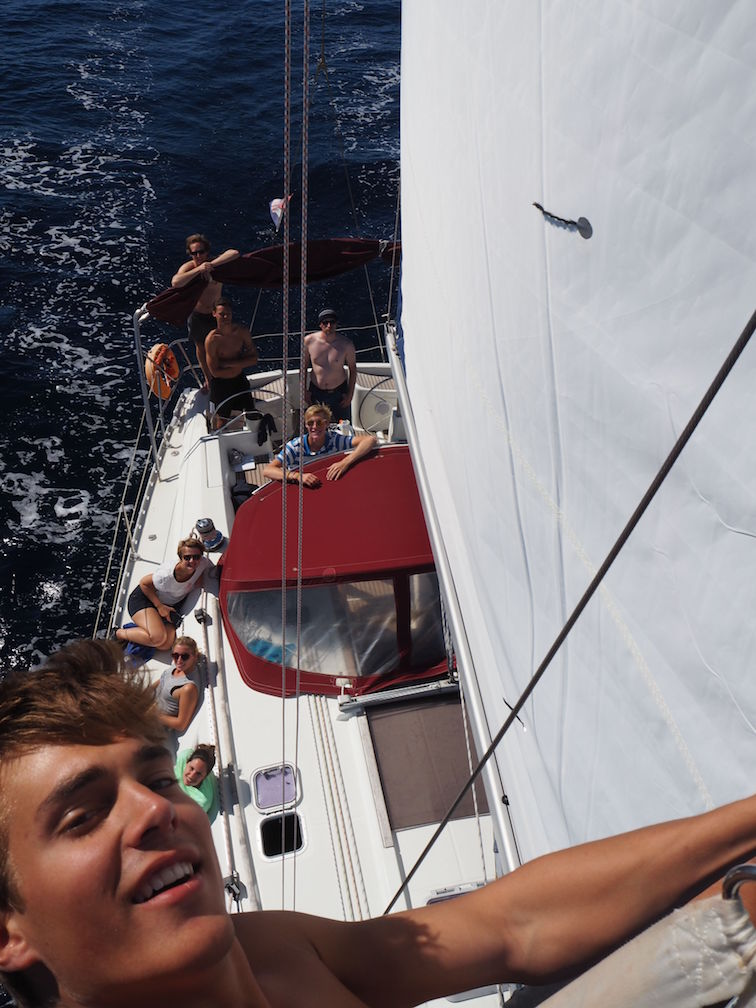
\includegraphics[width=0.435\textwidth]{rohmaterial-bilder/segeln.jpg}
    \end{center}
    \caption[Segeltörn mit dem USCU]{Segeln ist ein \glq wissenschaftlicher Sport\grq.}
  \end{wrapfigure}

Universitätspräsident Professor Michael Weber lobte in seinem Grußwort die außergewöhnliche Nachwuchsarbeit und dankte dem Verein für dessen erfolgreiche Außenwerbung. \glqq Segeln ist ein sehr wissenschaftlicher Sport. Hier kommen Leben, Lernen und Forschen zusammen\grqq, betonte der Präsident. Außerdem fördere das Segeln - wie von Hoppe bereits erwähnt - die Entwicklung persönlicher Fähigkeiten, darunter gerade auch solche, die in der Wissenschaft wichtig seien wie Mut, Ausdauer und Problemlösungskompetenz. 

Bei der Feier präsentierte sich auch der Shanty-Chor des USCU mit traditionellen Seemannsliedern, ganz klassisch begleitet mit Gitarre und Akkordeon. Und wie es sich laut Satzung für die „Commodores“ gehört, kamen die langjährigen ehemaligen Vereinsvorsitzenden Dr. Klaus Murmann und Professor Harald Traue ihren Repräsentationspflichten nach. Murmann, der gebürtige Füssener, der als Mitarbeiter in der Servicegruppe Informatik arbeitet, ist seit 1977 im Verein und übernahm gleich im ersten Jahr Verantwortung als Vorsitzender. Anekdotenreich rollte er in seiner Rede Seemannsgarn aus der Vereinsgeschichte auf und wusste vor allem von den Ausbildungstörns viel Amüsantes zu berichten. 

Harald Traue, der bis zu diesem Jahr als Professor die Sektion für Medizinische Psychologie leitete, kam 1989 zum USCU und war dreiundzwanzig Jahre lang Vorsitzender des Vereins. Der Wissenschaftler widmete sich in seiner Rede der anthropologischen und psychologischen Bedeutung des Segelns. Warum begibt man sich als Mensch ohne Not und Notwendigkeit auf das Wasser? Überflüssig, anstrengend und meistens dazu nass und kalt sei diese Tätigkeit. Traue sprach von den „healthy pleasures“, also vom gesunden Vergnügen, und erklärte die Faszination Segeln mit etwas Urmenschlichem, nämlich der ungeheuren Lust, auf das bewegte Wasser zu schauen. Und noch ein fundamentales Bedürfnis stille der Segelverein: das Bedürfnis nach Zusammenhalt in einer selbstlosen Gemeinschaft. „Unser Universitätssegelclub ist kein Profitcenter, sondern eine Solidargemeinschaft, die auch den Charakter ihrer Mitglieder prägt“, so der Commodore. Das kann auch an einer Universität nicht schaden. 

\cref{cha:2} ist auszugsweise dem Artikel in \cite[S. 54--56]{uni-ulm-intern} entnommen. Wir danken der Pressestelle der Universität Ulm für die freundliche Genehmigung der Verwendung von Text und Bild.